\documentclass[12pt, conference, onecolumn, draftclsnofoot]{IEEEtran}
\IEEEoverridecommandlockouts
% The preceding line is only needed to identify funding in the first footnote. If that is unneeded, please comment it out.
\usepackage{cite}
\usepackage{amsmath,amssymb,amsfonts}
\usepackage{algorithmic}
\usepackage{graphicx}
\usepackage{textcomp}
\usepackage{xcolor}
\usepackage{float}
\usepackage{setspace}
\def\BibTeX{{\rm B\kern-.05em{\sc i\kern-.025em b}\kern-.08em
    T\kern-.1667em\lower.7ex\hbox{E}\kern-.125emX}}
\begin{document}

\title{GNSS in the Classroom: Taking the Paralysis out of Analysis - Abstract}

\author{\IEEEauthorblockN{Andrew Neish}
\IEEEauthorblockA{\textit{Aeronautics and Astronautics} \\
\textit{Stanford University}\\
Stanford, USA \\
amneish@stanford.edu}
\and
\IEEEauthorblockN{Tyler Reid}
\IEEEauthorblockA{
\textit{Xona Space Systems}\\
San Mateo, USA \\
tyler@xonaspace.com}
\and
\IEEEauthorblockN{Frank van Diggelen}
\IEEEauthorblockA{\textit{Android Location} \\
\textit{Google}\\
Mountain View, USA \\
fvandiggelen@google.com}
\and
\IEEEauthorblockN{Grace Gao}
\IEEEauthorblockA{\textit{Aeronautics and Astronautics} \\
\textit{Stanford University}\\
Stanford, USA \\
gracegao@stanford.edu}
}

\begin{singlespace}
    \maketitle 
\end{singlespace}

Teaching any subject can be difficult, but teaching GNSS offers a unique set of challenges.
GNSS is built upon a set of complex and interdisciplinary engineering achievements. 
The modernization of these systems today continues to push the boundaries of orbital mechanics, material science, modern physics, rocket science, and a host of other fields.
But for all of the technological complexities of GNSS, it has turned into one of the most recognized and widely used utilities throughout the world.
Everyone has become a capable "Navigator" through the simple act of owning a cell phone.
So how does one boil all of this information down in to a 10 week graduate engineering course?
Furthermore, how does one go beyond giving students a theoretical background to give them the vocational tools necessary to innovate and carry the field of navigation forward?

At Stanford, the GPS course has always strived to achieve proficiency in the theory and practice.
The class has served as the inspiration to many who join the navigation profession and continue to lead in the field today.
With the emergence of the GNSS Analysis Tools from Google \cite{vanDiggelen2018}, many new opportunities have arisen that allow students to explore the world of GNSS by following their passions and their own creativity.
The GNSS Analysis Tools available on Android \cite{GNSSAnalysisTools}, allows anyone with an Android phone to record raw GNSS measurements.
By raw GNSS measurements, we're not simply referring to pseudoranges.
After all, a pseudorange is a derived measurement.
True raw measurements are comprised of the time stamps associated with satellite signal reception and transmission, AGC, $C$/$N_0$, and other values used to generate a position, velocity, and time (PVT) solution.
With these measurements available to the masses, everyone can tinker and toy with real GNSS data and the Stanford GPS course has wholeheartedly embraced these new tools.

Over the years, the course has been molded to enhance student engagement and encourage newcomers from diverse professional backgrounds. 
The goal has been to help them explore the intersection between their passions and GNSS.
As a project based course, students learn of the different subsystems while they develop their own personal projects using the GNSS Analysis Tools.
These projects can take inspiration from their current work and interests or they can be derived from any aspect of GNSS that piques their interest.
They benefit greatly from their lack of experience in the field as it frees them to explore ideas that many of us might not pursue ourselves.
Midway through the course, the students are prompted to create a project that uses the skills developed within the class and are given little direction during the initial brainstorming.
There is some scoping and guidance from the instructors as the course goes on, but these projects are largely born of the student's own volition.

This paper exhibits some of the projects that these students were able to accomplish in a mere matter of weeks.
An example project includes the use of neural networks to improve position estimates on trajectories with non-Gaussian noise \cite{LSTM2018}.
In this project, the authors were able to build and train a neural network to recognize simulated multipath error and then tested this network using real world data (See Figure \ref{LSTM}).

\begin{figure}[H]
    \centering
    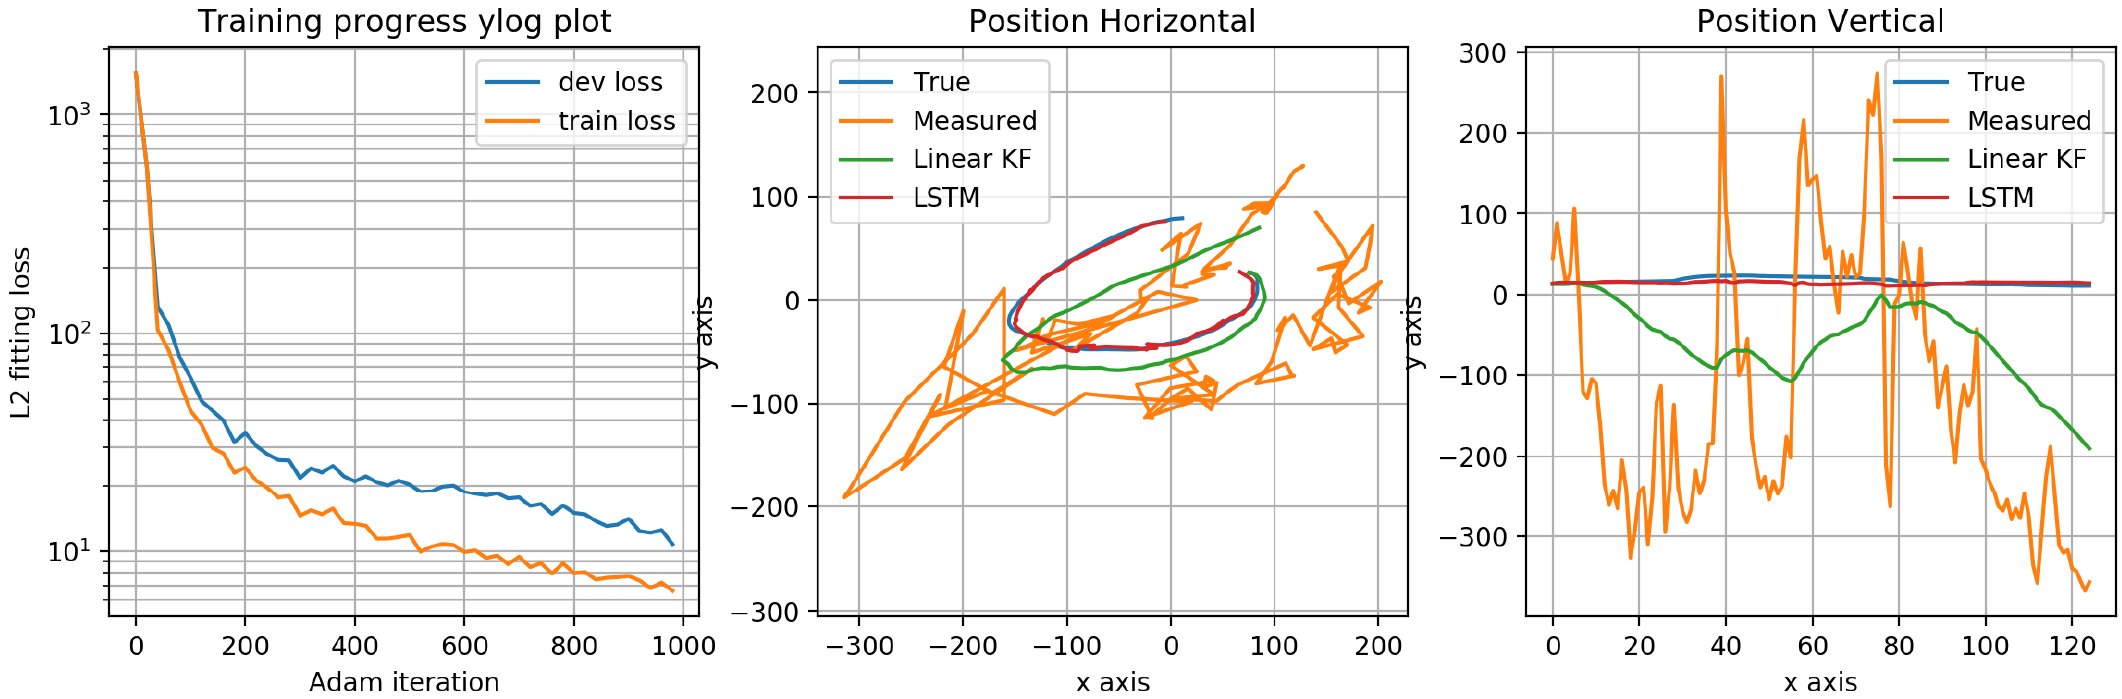
\includegraphics[width=6.5in, height=2.25in]{Figures/Mateh-LSTM.PNG}
    \caption{LSTM performance in multipath environments}
    \label{LSTM}
\end{figure}

In another project, the authors used building models to reconstruct non-line-of-sight (NLOS) pseudoranges from obstructed satellites and project those NLOS signals on to "virtual satellites" in an effort to construct a more accurate PVT solution \cite{NLOS2018} (See Figure \ref{NLOS}).

\begin{figure}[H]
    \centering
    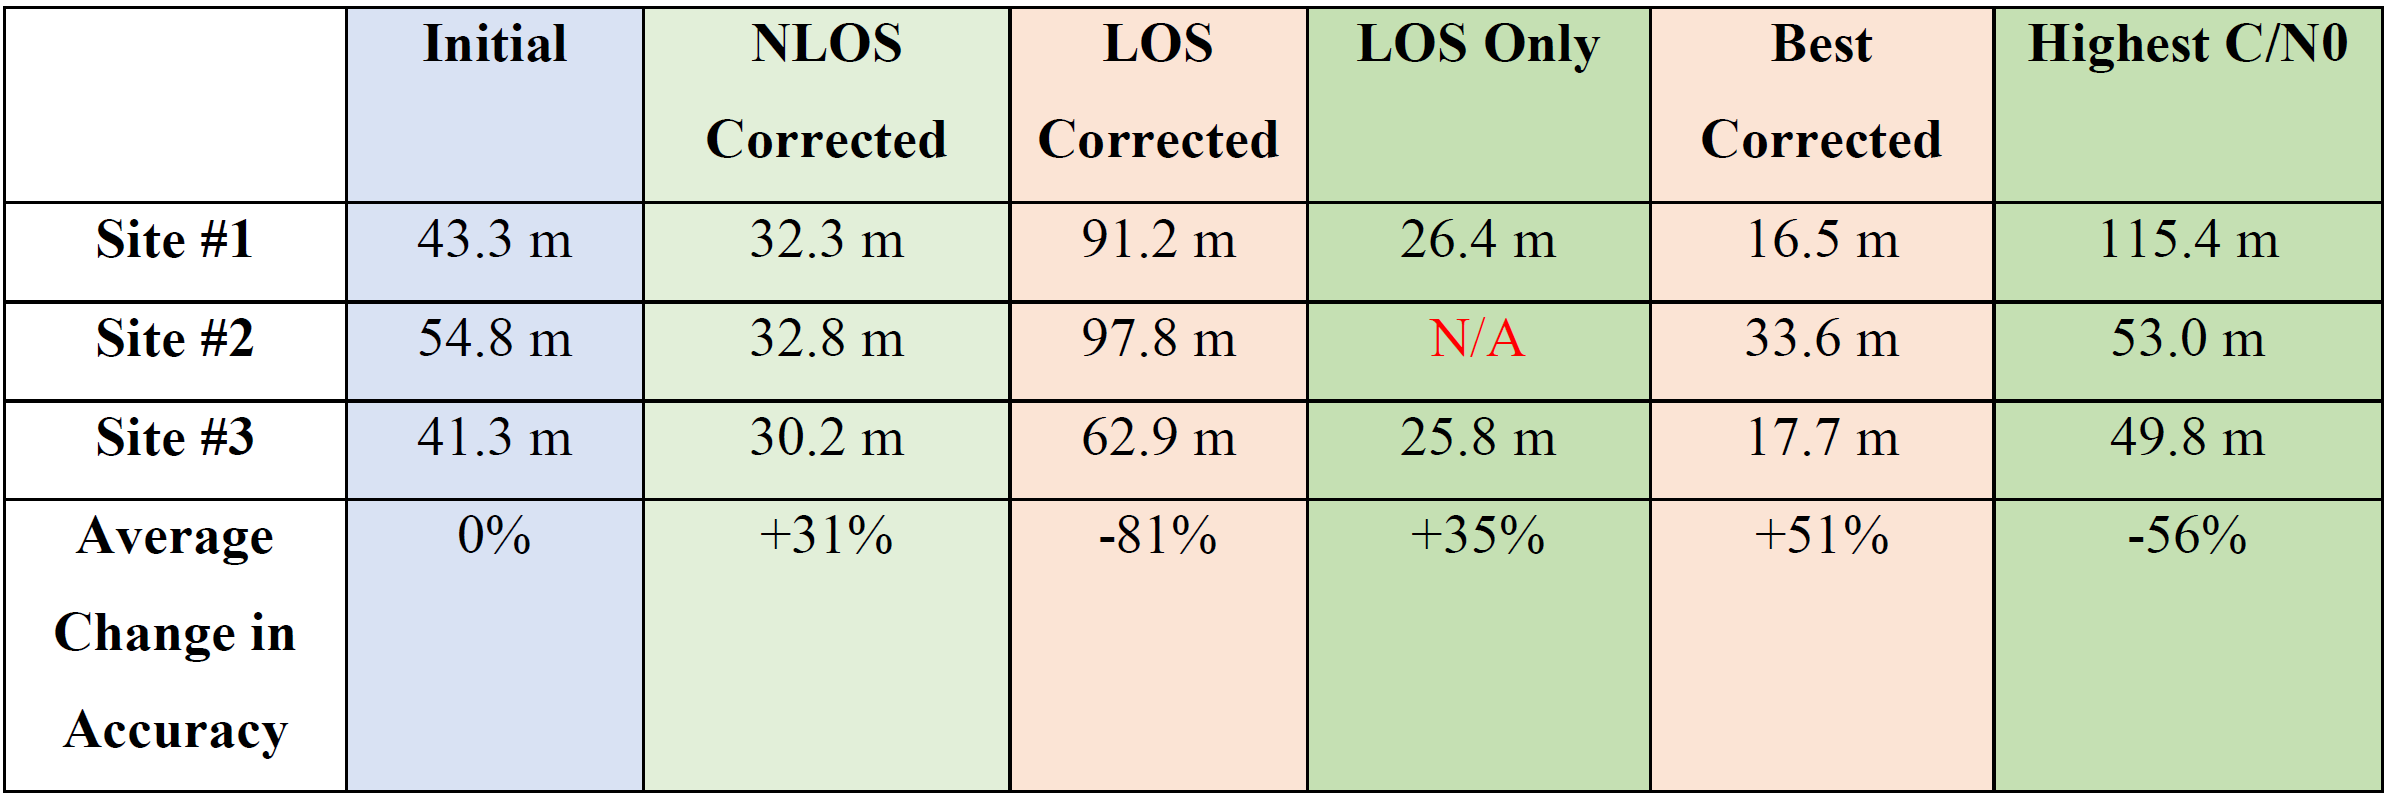
\includegraphics[width=6.5in, height=2.25in]{Figures/NLOS-Table.PNG}
    \caption{Position accuracies with NLOS corrections}
    \label{NLOS}
\end{figure}

These projects and more will be presented to highlight the promise these modern tools bring to project oriented teaching.
The goal of this paper is to serve as an inspiration to those teaching or considering teaching GNSS.
Whether instructing undergraduates, graduates, or professionals, this paper presents some of the opportunities that arise when students have a chance to creatively pursue GNSS themselves.

\begin{thebibliography}{00}
    \bibitem{vanDiggelen2018} Van Diggelen, Frank, and Mohammed Khider. "GNSS analysis tools from Google." Inside GNSS 13 (2018): 51. 
    \bibitem{GNSSAnalysisTools} https://github.com/google/gps-measurement-tools/releases/tag/2.0.0.1
    \bibitem{LSTM2018} Kosec, Matej, and John Poothokaran. "Comparison of Kalman filters and LSTM networks for GPS trajectory smoothing in the presence of simulated multipath noise." Stanford GPS Class (2018).
    \bibitem{NLOS2018} Pratz, Scott, and Riley Culberg. "NLOS Identification and Correction from Known Building Structures." Stanford GPS Class (2018).
    
\end{thebibliography}

\end{document}
